\chapter{Задание}
\section{Цель работы}
\textbf{Цель работы:} построение гистограммы и эмпирической функции распределения.
\section{Содержание работы}
\begin{enumerate}
	\item Для выборки объёма $n$ из генеральной совокупности $X$ реализовать в виде программы на ЭВМ
	\begin{enumerate}
		\item вычисление максимального значения $M_{\max}$ и минимального значения $M_{\min}$;
		\item размаха $R$ выборки;
		\item вычисление оценок $\hat\mu$ и $S^2$ математического ожидания $MX$ и дисперсии $DX$;
		\item группировку значений выборки в $m = [\log_2 n] + 2$ интервала;
		\item построение на одной координатной плоскости гистограммы и графика функции плотности распределения вероятностей нормальной случайной величины с математическим ожиданием $\hat{\mu}$ и дисперсией $S^2$;
		\item построение на другой координатной плоскости графика эмпирической функции распределения и функции распределения нормальной случайной величины с математическим ожиданием $\hat{\mu}$ и дисперсией $S^2$.
	\end{enumerate}
	\item Провести вычисления и построить графики для выборки из индивидуального варианта.
\end{enumerate}


\chapter{Теоретическая часть}
\section{Формулы для вычисления величин $M_{max}$ , $M_{min}$, $R$, $\hat\mu$, $S^2$}

Пусть $\vec{x} = (x_1, \dots, x_n)$ --- выборка из генеральной совокупности Х, где $n$ --- объём данной выборки.
Расположим компоненты $x_i$, $i=\overline{1,n}$ в порядке неубывания: 
\begin{equation}
	\label{eq:leq}
	x_{(1)}~\leq~x_{(2)}~\leq~\dots~\leq~x_{(n)}
\end{equation}

Вариационным рядом, построенным по выборке $\vec{x} = (x_1, \dots, x_n)$, называют вектор $(x_{(1)}, \dots, x_{(n)})$.

Минимальное значение выборки рассчитывается по формуле (\ref{eq:min}); максимальное --- (\ref{eq:max}). Размах выборки рассчитывается по формуле (\ref{eq:diff}); выборочное среднее --- (\ref{eq:mx}), исправленная выборочная дисперсия --- (\ref{eq:dx}).
\begin{equation}
	\label{eq:min}
	M_{\min} = x_{(1)} = \underset{x_i \in \vec{x}}{min}~x_i
\end{equation}
\begin{equation}
	\label{eq:max}
	M_{\max} = x_{(n)} =  \underset{x_i \in \vec{x}}{max}~x_i
\end{equation}
\begin{equation}
	\label{eq:diff}
	R = M_{\max} - M_{\min}.
\end{equation}
\begin{equation}
	\label{eq:mx}
	\hat\mu(\vec x) = \frac 1n \sum_{i=1}^n x_i
\end{equation}
\begin{equation}
	\label{eq:dx}
	S^2(\vec x) = \frac 1{n - 1} \sum_{i=1}^n (x_i - \hat\mu)^2
\end{equation}


\section{Эмпирическая плотность и гистограмма}
Пусть $\vec{x} = (x_1, \dots, x_n)$ --- реализация выборки из генеральной совокупности $X$, где $n$ --- объём данной выборки.

При большом объеме n выборки  значения $x_i$ группируют в интервальный статистический ряд. Для этого отрезок $J = [x_{(1)}, x_{(n)}]$ делят на $m$ равновеликих промежутков по формуле (\ref{eq:ji}):

\begin{equation}
	\label{eq:ji}
	J_i = [x_{(1)} + (i - 1) \cdot \Delta,\ x_{(1)} + i \cdot \Delta), i = \overline{1; m - 1}
\end{equation}
Последний промежуток определяется по формуле (\ref{eq:jm}):
\begin{equation}
	\label{eq:jm}
	J_{m} = [x_{(1)} + (m - 1) \cdot \Delta, x_{(n)}]
\end{equation}

Ширина каждого из таких промежутков определяется по формуле (\ref{eq:delta}).
\begin{equation}
	\label{eq:delta}
	\Delta = \frac{|J|}{m} = \frac{x_{(n)} - x_{(1)}}{m}
\end{equation}

Интервальным статистическим рядом, отвечающим выборке $\vec{x}$, называют таблицу \ref{table:row1}, в которой $n_i$ --- число элементов выборки, попавших в $J_i$, $i=\overline{1,m}$

\begin{table}[ht!]
	\captionsetup{singlelinecheck = false, justification=centering}
	\caption{Интервальный статистический ряд}
	\centering
	\label{table:row1}
	\begin{tabular}{|c|c|c|c|c|}
		\hline
		$J_1$ & ... & $J_i$ & ... & $J_m$ \\
		\hline
		$n_1$ & ... & $n_i$ & ... & $n_m$ \\
		\hline
	\end{tabular}
\end{table}

Пусть для выборки $\vec{x} = (x_1, \dots, x_n)$ построен интервальный статистический ряд ($J_i$, $n_j$), $i=\overline{1,m}$.

\textbf{Эмпирической плотностью}, отвечающей выборке $\vec x$, называют функцию:
\begin{equation}
	f_n(x) =
	\begin{cases}
		\frac{n_i}{n \Delta}, x \in J_i, i = \overline{1; m} \\
		0\ \ , x \not\in J \\
	\end{cases}
\end{equation}

где $J_i$ --- полуинтервал статистического ряда, 
$n_i$ --- количество элементов выборки, входящих в полуинтервал.

\textbf{Гистограмма} --- это график эмпирической функции плотности. 


\section{Эмпирическая функция распределения}

Пусть $\vec{x} = (x_1, \dots, x_n)$ --- выборка из генеральной совокупности $X$, где $n$ --- объём данной выборки.
Обозначим $l(t, \vec x)$ --- число элементов выборки $\vec x$, которые имеют значения меньше $t$.

\textbf{Эмпирической функцией распределения}, отвечающей выборке $\vec x$, называют отображение $F_n: R \to R$, определенное правилом: 

\begin{equation}
	F_n(t) = \frac{l(t, \vec x)}{n}
\end{equation}


\chapter{Практическая часть}

\section{Результаты расчетов}
\textbf{Индивидуальный вариант №14}

Результаты расчетов для выборки приведены на формулах (\ref{eq:res_min}), (\ref{eq:res_max}), (\ref{eq:res_r}), (\ref{eq:res_mx}), (\ref{eq:res_dx}), (\ref{eq:res_m}).
\begin{equation}
	\label{eq:res_min}
	M_{\min} = 0.09
\end{equation}
\begin{equation}
	\label{eq:res_max}
	M_{\max} = 5.47
\end{equation}
\begin{equation}
	\label{eq:res_r}
	R = 5.38
\end{equation}
\begin{equation}
	\label{eq:res_mx}
	\hat\mu(\vec x) = 3.055
\end{equation}
\begin{equation}
	\label{eq:res_dx}
	S^2(\vec x) = 1.055
\end{equation}
\begin{equation}
	\label{eq:res_m}
	m = 8
\end{equation}

На рисунке \ref{image:graph1} представлены гистограмма и график функции плотности распределения вероятностей нормальной случайной величины с выборочным математическим ожиданием $\hat\mu$ и выборочной дисперсией $S^2$.
\begin{figure}[h]
	\centering{
		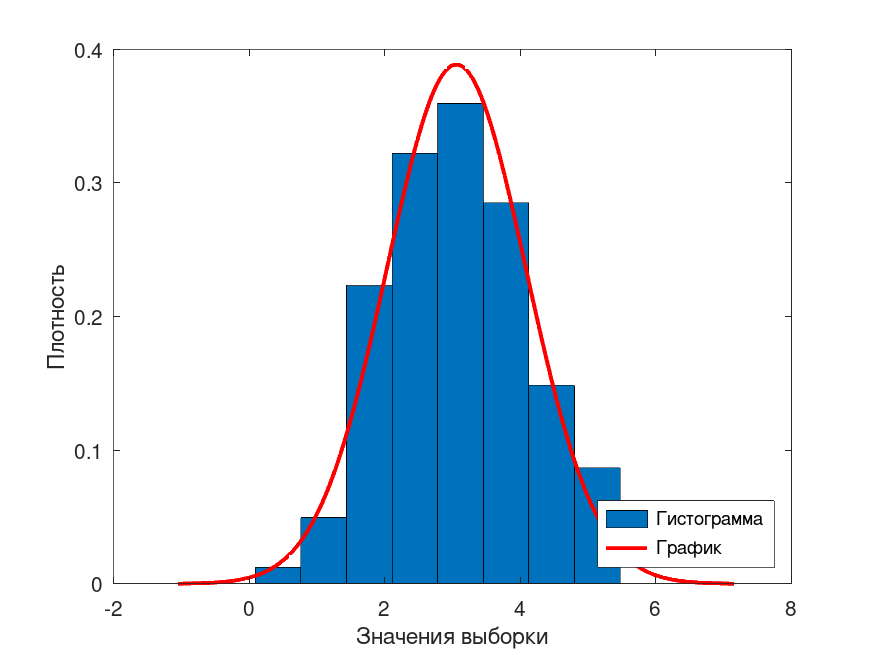
\includegraphics[scale=0.4]{./img/func_dp.png}
		\caption{Гистограмма и график функции плотности распределения вероятностей.}
		\label{image:graph1}
	}
\end{figure}

\clearpage

На рисунке \ref{image:graph2} представлены график эмпирической функции распределения и функции распределения нормальной случайной величины с выборочным математическим ожиданием $\hat\mu$ и выборочной дисперсией $S^2$.
\begin{figure}[h]
	\centering{
		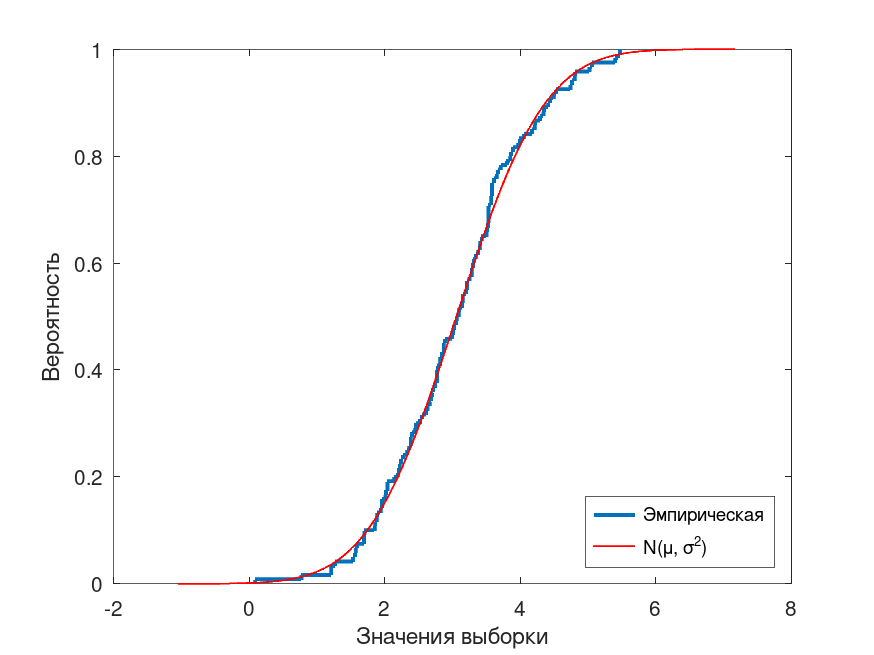
\includegraphics[scale=0.4]{./img/func_ep.png}
		\caption{Графики эмпирической функции распределения и функции распределения нормальной случайной величины.}
		\label{image:graph2}
	}
\end{figure}
